

\section{$P_N$-Solver}
\label{sec:pnsolver}

The truncation order $N$ is the key input parameter to the solver. With higher values, manually coding the solver from the equations would be ardous, error prone and very time consuming. We therefore decided to make use of the equations computer algebra representation and designed our solver around it.

The solver consists of two components. The first is a precomputation (section~\ref{sec:solver_precomputation}), which is done once for every single value of $N$. This steps runs a partial evaluation on the mathematical expression tree and applies the spatial discretization in a reference space we call stencil space. The precomputation step automatically generates source code from the resulting expression tree.

The generated stencil code is compiled with the runtime component (section~\ref{sec:solver_runtime}) of our solver. This component gets the actual problem as input, including gid resolution and RTE parameter fields. It builds the linear system and solves it using standard methods. An overview of the solver is given in figure~\ref{fig:pnsolver}.

\begin{figure*}[t!]
\centering
%\missingfigure{$P_N$-solver overview: generate stencil code $\rightarrow$ build system $\rightarrow$ solve $\rightarrow$ render}
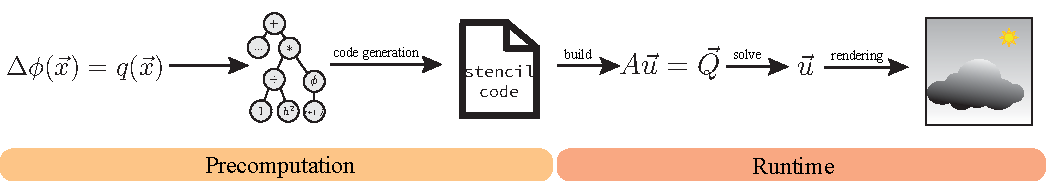
\includegraphics[width=\textwidth]{figures/fig_pipeline.pdf}
\vspace{-0.2in}
\icaption{Overview of our $P_N$-solver. After generating the stencil source code from the expression trees representing the $P_N$-equations, the linear system $A\vec{u}=\vec{Q}$ is built using RTE parameter fields and additional user input, such as grid resolution and type of boundary conditions. The resulting system is solved for $\vec{u}$, which is then used in our rendering application.}
\label{fig:pnsolver}
\end{figure*}

\subsection{Precomputation}
\label{sec:solver_precomputation}

The result of the precomputation is a stencil, which can be used during runtime to build the linear system for a given problem. The stencil is a pattern of indices into the solution vector, along with some weights. It expresses how the sum of the weighted solution vector components relate to the RHS for a given unknown in the system and therefore contains most information required to propagate a row in the system matrix $A$ and RHS-vector $\vec{Q}$. The index pattern does not change for different rows, giving the stencil its name.

A stencil generally is crafted by discretizing a PDE at a hypothetical center voxel $ijk$ (assuming to mean the voxel center most of the time). Finite differences create weighted references to other voxels (e.g. $i+1,jk$). After bringing the discretized equation into canonical form (a weighted sum of unknowns), one can write the stencil by reading off the weights and $ijk$-offsets. $ijk$ will only be known during runtime, when the stencil is executed for a particular unknown (row). Then the offsets can be used to find the component index into the solution-vector and weights can be evaluated for concrete world space position. We refer to the space with the hypthetical voxel $ijk$ at the center as stencil space.

Typically, the stencil is coded by hand, which would be challenging with our $P_N$-equations and higher values of $N$. In our system, the stencil code is created automatically from the computer algebra representation. Spatial discretization and fatorization into canonical form are done as manipulation passes on the mathematical expression tree. The precomputation code iterates over all terms and analyzes the unkown to get the $ijk$-offset. The factor-expression is extracted from the tree and used to generate source code for evaluating the factor-expression during runtime (including calls for evaluating RTE-parameter fields).

The spatial discretization is done by parsing the expression tree of each equation from the root. All occurances of the continuous positional variable $\vec{x}$ are replaced by discrete voxel coordinates $i,j,k$, whose values are retrieved from the top of a stack. The stack is kept by the parser and is initialized with the voxel at $ijk=(0,0,0)$.

Whenever the parser encounters a differential operator, the current voxel position is shifted and pushed to the stack. Then the child expression is parsed and multiplied with a weight value, followed by popping the stack. This is done for each element of a central difference stencil, which provides the offset and weight values (referencing the voxelsize variable). The dimension of the stencil is given by the derivation variable of the operator. Nested derivatives are handled naturally and produce higher order finite difference stencils as expected.

Another aspect to consider during discretization is the location of the variables and unknowns. As we will see later, our solver needs to support staggered grids, where the SH coefficients are not all located at the voxel center (collocated). Coefficients can also be located at face-centers, edges and intersections of voxels (staggered).

Our solver supports placement of coefficients at arbitrary staggered grid locations. Whenever a coefficient is encountered during expression tree parsing for discretization, the parser checks how its location is related to the current location on the top of the stack. Depending on how the two are located to each other, the parser returns an expression, which interpolates the coefficients at the requested offset from its surrounding locations, or it returns the coefficient itself, if it happens to coincide. This is also done for RTE parameters, such as $\sigma_t$ or $p^{l,m}$, which are always located at the voxel center. The position stack of the parser is initialized with the staggered grid location defined by the coefficient, which is associated with the $l,m$-pair of the equation currently being discretized.

%\subsection{Stencil Code Generation}

% After applying the discretization step to the expression tree of the $P_N$-equations, it is used to generate the stencil code. In numerical analysis, a stencil is an arrangement of voxels and weights, that relate values at different locations to each other and form the basis for propagating rows in the system matrix $A$ and RHS vector $\vec{Q}$ with values. The name comes from the fact, that the geometric structure and weights of the configuration do not change, when applied to different voxels. The same is true for the $P_N$-equations and we use this fact to generate a single function, which propagates rows in $A$ and $\vec{Q}$ for a given voxel.

%The $P_N$-equations express, how each coefficient of a voxel depends on other coefficients of the same or adjacent voxels. The unknowns in the terms give information about the coefficient index and voxel offset, and therefore identify a column offset in the matrix $A$. The factors to these coefficients may contain evaluations of RTE parameters, such as $\sigma_t$. Therefore, these factors can not be determined during stencil generation, but are rendered into code expressions, which are executed as part of the stencil function during runtime. Because the stencil code has been generated in stencil space relative to the voxel at $(0,0,0)$, we can run the same stencil code for every voxel, by simply applying an offset accordingly. 



%\subsection{System Building and Solving}
\subsection{Runtime}
\label{sec:solver_runtime}

The generated stencil code is generated once for every value of $N$ and compiled with the runtime component of our solver. The runtime executes the stencil for every voxel to propagate the system matrix $A$ and RHS vector $\vec{Q}$ with numerical values.

The number of rows is determined by the number of voxels times the number of coefficients per voxel (see figure~\ref{fig:matrix_layout}) and can therefore become very large for high resolution and high truncation order. The matrix $A$ is squared and fortunately very sparse, due to finite differences and the structure of the $P_N$-equations. Unfortunately, it also is non-symmetric (due to the transport term) and not diagonal dominant, which rules out many standard methods for solving linear systems. We adress this by solving the normal form $A^TA\vec{u}=A^T\vec{Q}$ instead. This gives a symmetric and positive definit system matrix $A^TA$, albeit with a higher condition number.


The $P_N$-equations have been discretized, and the stencil has been generated, without any notion of domain boundaries and boundary conditions (BC). Our solver supports Neumann BC and Dirichlet BC. They are handled transparently by the code which runs the stencil. Whenever the stencil writes into $A$ for a boundary coefficient, the framework will either ignore the write operation (Dirichlet BC) or write into the row and column in $A$ of the coefficient in the closest voxel inside the domain (Neumann BC).

In order to respect the boundary correctly, additional coefficients (which contribute additional rows and columns in $A$ and $\vec{Q}$) are necessary at boundary voxels (see Figure~\ref{fig:staggeredgrid}). This requires careful managegment and bookkeeping of coefficient indices, which is done transparently by the runtime code.




\begin{figure}[h]
\centering
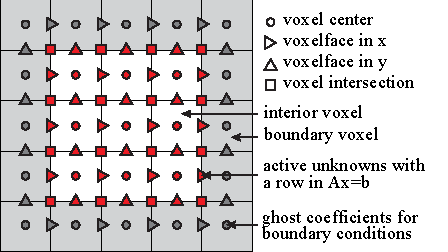
\includegraphics[width=0.5\columnwidth]{figures/fig_staggered_grids.pdf}
%\vspace{-0.2in}
\icaption{Staggered grids place coefficients at different locations within the finite difference grid. Additional unknowns are required in boundary cells to produce a correct result.}
\label{fig:staggeredgrid}
\end{figure}

%\begin{figure}[h]
%\centering
%\begin{subfigure}{0.45\columnwidth}
%%\missingfigure{test}
%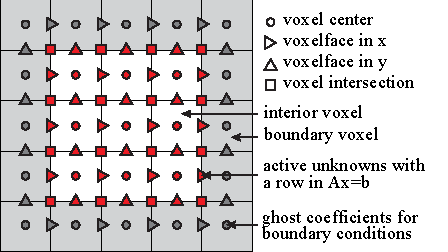
\includegraphics[width=\columnwidth]{figures/fig_staggered_grids.pdf}
%\end{subfigure}%
%\hspace{0.05\columnwidth}
%\begin{subfigure}{0.45\columnwidth}
%\missingfigure{test2}
%\end{subfigure}%
%\vspace{-0.2in}
%\icaption{Staggered grids cause a shifted boundary on the right and upper side of the domain (left). The boundary is correct after introducing additional unknowns (red) at boundary voxels (right).}
%\label{fig:staggeredgrid}
%\end{figure}


%Matrix $A$ and vector $\vec{Q}$ are constructed after applying the stencil for every voxel.



%\subsection*{CDA vs. $P_1$}
%\begin{itemize}
  %\item CDA is a degenerated form of $P_1$. It is derived by isolating the flux-vector on one side of the vector-equation formed by the $l=1$ SH-band equations. This isolation requires division by the extinction coefficient, introducing a $\frac{1}{\sigma_t}$ factor which diverges as $\sigma_t$ approaches zero. Thresholding to some minimum is required, in order to be able to solve the system for vacuum regions.
  %\item $P_1$ does not require any thresholding of $\sigma_t$ as it does not contain $\sigma_t$ as a denominator. It therefore can deal with vacuum regions without modifications.
  %\item (needs validation) Further, in the presence of vacuum or near vacuum regions, the condition number for CDA is higher than for $P_1$, because of small extinction values in the denominator of the diffusion coefficient.
  %\item Using the normal form for CDA will further increase the condition number when vacuum regions are present and significantly decreases convergence.
%\end{itemize}

